\UseRawInputEncoding
\documentclass[a4paper,openany,12pt]{book}
\usepackage[spanish, es-ucroman]{babel}
\usepackage[utf8]{inputenc}
\usepackage{fancyhdr}
\usepackage{graphicx}
\usepackage[inner=3.0cm,outer=2.5cm,top=3cm,bottom=3cm]{geometry}%margen 2.54
\usepackage{hlundef}
\usepackage{tesis}
\usepackage[printonlyused]{acronym}
\usepackage{breakcites}
\usepackage{color,soul}
\usepackage{ae}
\usepackage[usenames,dvipsnames,table,xcdraw]{xcolor}
\usepackage{amsmath}
\usepackage{multirow}
\usepackage[inline]{enumitem}
\usepackage{tikz,pgfplots,pgfplotstable}
\usepackage{capt-of}
\usepackage{csvsimple}
\usepackage[breaklinks]{hyperref}
\setlength{\parindent}{1.27cm}
\usepackage[acronym]{glossaries} % paquete de acrónimos
\usepackage{caption}
%\usepackage{subcaption}
\usepackage{booktabs}
\usepackage{enumitem}
\usepackage[colorinlistoftodos]{todonotes}
\usepackage{mathrsfs}
\newtheorem{proposicion}{Proposición}[section]
\usepackage{amsfonts}
\usepackage{etoolbox}
\usepackage[group-separator={,}]{siunitx}
\usepackage{graphicx} 
\usepackage{adjustbox} % también para rotar
\usepackage{array} % Para definir ancho tabla
\usepackage{booktabs}
\newcommand{\ra}[1]{\renewcommand{\arraystretch}{#1}}
\setcounter{secnumdepth}{3}
\pgfplotsset{compat=1.13}
\usepgfplotslibrary{colormaps}
\usepackage{sidecap}
\sidecaptionvpos{figure}{b}
\sidecaptionvpos{table}{b}
\usepackage{natbib}
\setcitestyle{round}
\usepackage{tikz-qtree}
\usepackage{arydshln}
\usetikzlibrary{shapes.geometric, arrows, decorations.pathreplacing, shadows,trees, positioning, calc, tikzmark, spy, mindmap, matrix}
\tikzstyle{roundedFrame} = [rectangle, text centered, rounded corners, draw=gray]
\tikzstyle{input} = [rectangle,text centered, draw=none]
\tikzstyle{emptyFrame} = [rectangle,text centered, draw=white]
\tikzstyle{frame} = [rectangle, text centered, draw=gray]
\tikzstyle{arrow} = [thick,->,>=stealth]
\usepackage{pifont} % DING
% código para sacar el encabezado de chapter
\usepackage[T1]{fontenc}
\usepackage{titlesec, blindtext, color}
\definecolor{gray75}{gray}{0.75}
\newcommand{\hsp}{\hspace{20pt}}
\titleformat{\chapter}[hang]{\Huge\bfseries}{\thechapter\hsp\textcolor{gray75}{|}\hsp}{0pt}{\Huge\bfseries}
% Nuevos comandos para diagrama de gantt
% A package which allows simple repetition counts and some useful commands
\usepackage{forloop}
\newcounter{loopcntr}
\newcommand{\rpt}[2][1]{%
  \forloop{loopcntr}{0}{\value{loopcntr}<#1}{#2}%
}
\newcommand{\on}[1][1]{
  \forloop{loopcntr}{0}{\value{loopcntr}<#1}{&\cellcolor{gray75}}
}
\newcommand{\off}[1][1]{
  \forloop{loopcntr}{0}{\value{loopcntr}<#1}{&}
}
\usepackage[nottoc]{tocbibind}

% Para definir ancho tabla
\newcolumntype{L}{>{\centering\arraybackslash}m{4cm}} 
\usepackage[caption=false]{subfig}
%\input{colors.tex}
\usepackage{dsfont}
\usepackage{gantt}
\usepackage[ruled,vlined]{algorithm2e}

\newtheorem{defn}{Definition}[section]
\pagenumbering{Roman}

\title{``TÍTULO DE LA TESIS""}
\author{Br. NOMBRE COMPLETO DEL AUTOR}
\orientador{Dr./M.Cs./Ing. NOMBRE DEL ASESOR}
\coorientador{Dr./M.Cs./Ing. NOMBRE DEL CO-ASESOR (de ser el caso)}

\begin{document}
%%%%%%%%%%%%%%%%%%%%%%%%%%%%%%%%%%%%%%%%%%%%%%%%%%%%%%%%%%%%%%%%%%%%
% Compone la carátula, el resumen y abreviaturas de ser el caso
\maketitle
%%mayores detalles de como usas las abreviaturas (acronimos)
% vea: http://www.ctan.org/tex-archive/macros/latex/contrib/acronym/
% hay un manual en pdf en esa misma direccion

\chapter{Abreviaturas}
\printglossary[type=\acronymtype]
\newacro{gcd}{GCD}{Greatest Common Divisor}

\printglossary
\begin{acronym}

\ac{CPD}{Closest Pair Distance}
\acro{DTW}{Dynamic Time Warping}
\acro{ED}{Euclidean Distance}
\acro{GPS}{Global Positioning System}
\acro{IBM}{International Business Machines}
\acro{INEI}{Instituto Nacional de Estadística e Informática del Perú}
\acro{LCSS}{Longest Common Sub-Sequence}
\acro{NN}{Nearest Neighbors}
\acro{SHNN-CAD}{Sequential Hausdorff Nearest-Neighbor Conformal Anomaly Detector}
\acro{SOM}{Self Organized Map}
\acro{STI}{Sistema de Transporte Inteligente}
\acro{SPD}{Sum of Pair Distance}
\acro{t-SNE}{t-Distributed Stochastic Neighbor Embedding}
\end{acronym}

\begin{resumen}
%Aquí deberás colocar entre 100 y 150 palabras como máximo, el problema que intentas resolver, la justificación y los aportes o soluciones que planteas.
\noindent
Debe contener el tema de investigación, su importancia, los objetivos propuestos, las estrategias metodología y posibles aplicaciones. Debe ser redactado en un solo párrafo y no contener espacios entre líneas ni sangrías. Presentación: máximo 400  palabras, letra Arial 12, espacio sencillo (más información ver guía).

\end{resumen}
 %Inserta el resumen

%%%%%%%%%%%%%%%%%%%%%%%%% list of content %%%%%%%%%%%%%%%%%%%%%%%%
\tableofcontents %Inserta el índice general
\listoftables %Inserta el índice de cuadros
\addcontentsline{toc}{chapter}{Lista de Tablas}
\listoffigures %Inserta el índice de figuras
\addcontentsline{toc}{chapter}{Lista de Figuras}

\setlength{\tabcolsep}{6pt} % Default value: 6pt Horizontal spacing
\renewcommand{\arraystretch}{1}% Default value: 1 Vertical spacing
\clearpage
\pagenumbering{arabic}
%%%%%%%%%%%%%%%%%%%%%%%%%%%%%%%%%%%%%%%%%%%%%%%%%%%%%%%%%%%%%%%%%%%%%
% En esta parte deberás incluir los archivos de tu plan de tesis %%%%
%%%%%%%%%%%%%%%%%%%%%%%%%%%%%%%%%%%%%%%%%%%%%%%%%%%%%%%%%%%%%%%%%%%%%
\chapter{Antecedentes}
%En esta sección se va desde aspectos generales a  aspectos específicos (como un embudo). No se olvide que es la primera parte que tiene contacto con el lector y que hará que este se interese en el tema a investigar.
%El objetivo de esta sección es llevar al lector hacie el tema que se va a tratar en forma específica y dejar la puerta abierta a otras investigaciones.


\section{Trabajos Relacionados}

Antecedentes o esbozo del estado del arte. Reflejan los avances y el Estado actual del conocimiento en un área determinada y sirve de modelo o ejemplo para futuras investigaciones. Se refieren a todos los trabajos de investigación que anteceden a nuestro, es decir, aquellos trabajos donde se hayan manejado las mismas variables o se hallan comparaciones y tener ideas sobre cómo se trató el problema en esa oportunidad (dos a cuatro páginas - según guía) (más información ver guía).


Existen dos tipos de citaciones: citep y citet, los ejemplos a continuación respectivamente: \cite{lee2007trajectory} y \cite{roh2010nncluster}.
 %Inserta el capítulo 1
tr\chapter{Problema de Investigación}
Se espera que la descripción del problema sea amplia y detallada, se sugiere como mínimo tres páginas - según guía.

La problemática inicia cuando el sujeto detecta una necesidad concreta, falta de conocimiento o una contradicción entre los enfoques disponibles.

El problema de investigación se refiere a al descripción amplia y detallada de una realidad en la cual diversas variables o factores se relacionan, hechos-causas y consecuencias, y se concluye con una pregunta de investigación, que en esencia es la síntesis de la situación descrita. Es la conclusión a la que se llega después de haber descrito la situación problemática - Más información ver guía.

\section{Problema General}
Se sugiere que sea el titulo de la tesis en forma de pregunta. Se hace una pregunta la cual es respondida por la tesis. ¿Qué es lo difícil?


\section{Problemas Específicos}
(Se sugiere que sean pocos pero sustanciales)
El estudio toma en cuenta los siguientes problemas específicos:
\begin{itemize}
	\item Primer problema especifico.
	\item Segundo problema especifico.
	\item Tercer problema especifico.	
\end{itemize}
 %Inserta el capítulo 2
\chapter{Justificación}
La justificación  consiste en fundamentar la importancia del problema que aborda y la necesidad de realizar el trabajo práctico para hallar la solución al mismo.

La función principal es exponer las diferentes razones (impacto, beneficios, aportes teóricos, cambios o relevancias social) por las que es plausible llevar a cabo dicho trabajo - más información ver guía.
 %Inserta el capítulo 3
\chapter{Objetivos}
\section{Objetivo General}
El objetivo es un enunciado claro y preciso de lo que se persigue, debe responder a las preguntas ¿Qué? ¿ Para que? y ¿A través de que? (Se recomienda que el objetivo general este relacionado con el título)

\section{Objetivos Específicos}
Los objetivos deben ser metas concretas que pueden alcanzarse o no, pero que debe ser posible verificar cuando evalué el trabajo práctico. Es muy común confundir los objetivos con las tareas o con metas a largo plazo, o con resultados concretos que son parte de la investigación y no con su mera consecuencia.
(se recomienda que sean pocos objetivos específicos y que estén relacionados con los problemas específicos) (Se sugiere utilizar lista de verbos presentes en la guía)

 \begin{itemize}
	\item Primer objetivo específico
	\item Segundo objetivo específico
	\item Tercer objetivo específico
 \end{itemize} %Inserta el capítulo 4
\chapter{Hipótesis}

(Opcionalmente, una HIPÓTESIS de trabajo (QUE es lo que se deseas "probar") en caso de que la naturaleza del trabajo lo amerite).

Texto para introducir hipótesis

%\section{Tipo hipótesis}
 %Inserta el capítulo 5
\chapter{Alcances y Limitaciones}
(Se recomienda presentar los alcances y limitaciones en forma de puntos, se espera una redacción clara y detallada)

Los alcances y algunas limitaciones del estudio se presentan en los siguientes párrafos.

\section{Alcances}
Los alcances de este estudio pueden resumirse en:

 \begin{itemize}
 	\item Primer Alcance.
	\item Segundo Alcance.
	\item Tercer Alcance.
 \end{itemize}
\section{Limitaciones}

Algunas limitaciones de este estudio pueden resumirse en:

 \begin{itemize}
 	\item Primera limitación.
	\item Segunda limitación.
	\item Tercera limitación.
 \end{itemize}
  %Inserta el capítulo 6
\chapter{Marco Teórico}
(En este apartado el estudiante debe presentar en forma breve los temas que se abordarán en el marco teórico. El marco teórico se desprende de las palabras clave y del titulo. Debe ser totalmente acotado.
Ésta sección describe conceptos relacionados a procesamiento de trayectorias y detección de trayectorias anómalas .

\section{Primer subtitulo}
Aquí debe llenar tu contenido

\begin{algorithm}[H]
\SetAlgoLined
\KwData{$G=(X,U)$ such that $G^{tc}$ is an order.}
\KwResult{$G’=(X,V)$ with $V\subseteq U$ such that $G’^{tc}$ is an interval order.}
initialization\;
\nl \Begin{
\nl\While{not at end of this document}{
	\nl read current\;
	\nl \eIf{understand}{
	\nl go to next section\;
	\nl current section becomes this one\;
	}{
	\nl go back to the beginning of current section\;
	}
 }
 }
\caption{Ejemplo de como colocar código en código latex}
\label{IR2}
\end{algorithm}

Ejemplo para colocar citaciones: \cite{sillito2008semi}

Es posible utilizar abreviaturas dentro del contenido, abreviaturas como:
%\acronum{GPS}, \ac{INEI}, \ac{t-SNE}, \ac{SOM}, \ac{IBM}.

Para la utilización de ecuaciones matemáticas se puede utilizar el simbolo \$\$ dos veces tanto al inicio y al final, y para otros casos utilizar .

$$ E = mc^2 $$

Ecuaciones:
\begin{align*}
  1 + 2 &= 3\\
  1 &= 3 - 2
\end{align*}

Matrices: 
\[\begin{bmatrix}
1 & 0\\
0 & 1
\end{bmatrix}\]

otros:
\begin{equation}
(\frac{1}{\sqrt{x}})
\end{equation} %Inserta el capítulo 7
\chapter{Metodología}
(Se espera una redacción amplia y detallada la extensión esta determinada por el método seguido por el estudiante)
En este capitulo se presenta el tipo de metodología utilizado en esta tesis, así como las etapas que se seguirán para alcanzar los objetivos establecidos para la investigación.

\section{Tipo de Investigación}
Escribir que tipo de investigación se esta siguiendo.

\section{Métodos de Validación Propuestas}
Cuales serán las métricas utilizadas ?

% Insertando imagen.
  \begin{figure}
  \centering
  \subfloat[]{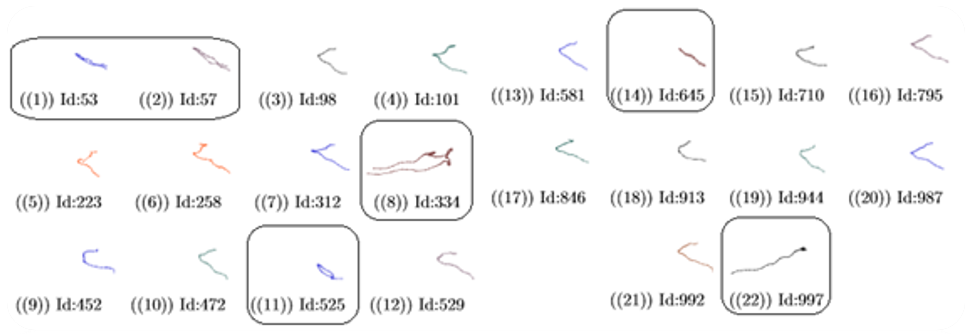
\includegraphics[width=150mm]{graficos/counting.png}}
  \caption[Ejemplo inserción de imagen]
  {Aquí deberas colocar la leyenda o descripción de la imagen.}
 % Nota. Adaptado de Título de la imagen, de Autor de la Imagen, año de publicación de la imagen, Fuente. Tipo de licencia.%
  \label{fig:counting}
  \end{figure}
% Fin insertando imagen

La metodología de investigación hace referencia al conjunto de procedimientos racionales y ordenados utilizados para alcanzar uno o varios objetivos que rigen en una investigación científica, en otras palabras, es el método utilizado para alcanzar los objetivos perseguidos. Se recomienda que el estudiante redacte en forma de párrafos el procedimiento a seguir para la elaboración de investigación.
 %Inserta el capítulo 8
\chapter{Resultados Esperados (a priori)}
El estudiante redactará los resultados que espera obtener al finalizar su proyecto o investigación.
 %Inserta el capítulo 9
\input{contenido/cap_10_comtribuciones_originales} %Inserta el capítulo 10
\chapter{Impacto Social Esperado}
El impacto social hace referencia a los efectos que el proyecto investigado tiene sobre la población en general por lo tanto, el estudiante deberá redactar el impacto social que espera tener su proyecto o investigación una vez finalizada, es decir, que región geográfica o sector de la población se va beneficiados.
 %Inserta el capítulo 11
\chapter{Índice Tentativo de Proyecto de Tesis}
(El estudiante propone un índice detallado que considere factible para la realización de investigación.)

\setlength{\tabcolsep}{3em} % for the horizontal padding
{\renewcommand{\arraystretch}{1.1}% for the vertical padding
\begin{tabular}{p{17cm}}

\noindent 
RESUMEN \\
CAPÍTULO I \\
1. INTRODUCCIÓN \\
\begin{enumerate}
	\item[1.1] Motivación y Contexto
    \item[1.2] Planteamiento del Problema
    	\begin{enumerate}
			\item[1.2.1] Problema General
			\item[1.2.2] Problemas Específicos
		\end{enumerate}
	\item[1.3] Objetivos
		\begin{enumerate}
			\item[1.3.1] Objetivo General
			\item[1.3.2] Objetivos Específicos
		\end{enumerate}
	\item[1.4] Contribuciones
	\item[1.5] Organización de la Tesis

\end{enumerate}

\end{tabular}

}

\setlength{\tabcolsep}{3em} % for the horizontal padding
{\renewcommand{\arraystretch}{1.1}% for the vertical padding
\begin{tabular}{p{17cm}}

CAPÍTULO II \\
2. MARCO TEÓRICO \\
\begin{enumerate}
	\item[2.1] Primer item
	\item[2.2] Segundo item
	
\end{enumerate}

CAPÍTULO III \\
3. TRABAJOS RELACIONADOS\\
\\
\\

CAPÍTULO IV \\
4. PROPUESTA \\
\begin{enumerate}
	\item[4.1] Arquitectura
	\item[4.2] Enfoque
	\begin{enumerate}
		\item[4.3.1] Preliminares
		\item[4.3.2] Segundo item
		\item[4.3.3] Tercer item
	\end{enumerate}
\end{enumerate}

\end{tabular}
}

\setlength{\tabcolsep}{3em} % for the horizontal padding
{\renewcommand{\arraystretch}{1.1}% for the vertical padding
\begin{tabular}{p{17cm}}

CAPÍTULO V \\
5. PRUEBAS Y RESULTADOS \\
\begin{enumerate}
	\item[4.1] Conjunto de Datos
	\item[4.2] Evaluación
	\item[4.3] Resultados
	
\end{enumerate}
CAPÍTULO VI \\
6. CONCLUSIONES Y TRABAJOS FUTUROS \\
\begin{enumerate}
	\item[6.1] Conclusiones
	\item[6.2] Trabajos Futuros
\end{enumerate}

ANEXOS \\
BIBLIOGRAFÍA \\

\end{tabular}

}
 %Inserta el capítulo 12
\chapter{Cronograma de Actividades}

\section{Linea de Tiempo}
(El impacto social hace referencia a los efectos que el proyecto investigado tiene sobre la población en general por lo tanto el estudiante deberá redactar el impacto social que espera tener su proyecto o investigación una vez  finalizada, es decir, que región geográfica o sector de la población se ven beneficiados.)

En esta sección listamos y explicamos las actividades planeadas en este proyecto. Además de explicar de forma detallada nuestra linea de tiempo para cada actividad. La Tabla \ref{fig:cronograma} muestra la relación de cada tarea con el tiempo en el que se ejecutará.

%\setlength{\tabcolsep}{6pt} % Default value: 6pt Horizoltal spacing
%\renewcommand{\arraystretch}{1}% Default value: 1 Vertical spacing

\section{Linea de Tiempo (segundo)}
El cronograma de actividades se muestra en la figura \ref{fig:cronograma}. 

\begin{figure}[!htb]
\caption{Diagrama de Gantt del cronograma de actividades.}
 \scalebox{0.8}{
  \begin{gantt}[xunitlength=1cm,fontsize=\small,titlefontsize=\small,drawledgerline=true]{9}{12}
    \begin{ganttitle}
      \titleelement{2016}{12}
    \end{ganttitle}
    \begin{ganttitle}
      \numtitle{1}{1}{12}{1}
    \end{ganttitle}
    \ganttbar[color=red]{\textbf{1. Revisión de la Literatura}}{1}{7}
    \ganttbar[color=red]{\textbf{2. Recolección de imágenes}}{4}{4}
    \ganttbar{\textbf{3. Presentación de plan de tesis}}{8}{1}
    \ganttbar{\textbf{4. Investigación de soluciones}}{8}{2}
    \ganttbar{\textbf{5. Implementación}}{10}{0.5}
    \ganttbar{\textbf{6. Evaluación}}{10.5}{0.5}
    \ganttbar{\textbf{7. Presentación de trabajo de tesis.}}{11}{1}    
  \end{gantt}
  }
  \label{fig:cronograma}
\end{figure}
 %Inserta el capítulo 13
\chapter{Presupuesto}

( Son los recursos necesarios para cubrir la investigación. Se refiere al estimado de la inversión total (compra de materiales si es necesario, movilización y otros gastos). Es recomendable señalar fuentes de financiamiento. )

En esta sección describiremos los recursos más importantes para el desarrollo de nuestra investigación.


\begin{table}[h] 
    \centering
    \scalebox{0.65}{
    \begin{tabular}{cccc}
        Tipo de Recurso & Nombre & Descripción & Costo  \\
        \midrule
        Hardware& Computador &  procesador i7     & 1,299.00   \\
                             & 					  &  memoria RAM 16GB               & 690.00    \\
                             & 					  &  placa madre Gigabyte           & 545.00    \\
                             &  				  &  tarjeta gráfica GTX 1070 8GB & 2,049.00  \\
        \hline
        Administrativos & Impresiones y pagos & impresión de documentos, impresión    & 600.00  \\
                        &                       & de tesis, copias de proyecto de tesis     &         \\
                        &                       & pago por inscripción de tesis, pagos    &         \\
                        &                       & por tramites administrativos              &         \\
        \hline
        Movilidad & Pasajes & gasto estimado en transporte & 200.00  \\
        \hline
        Otros     &         & gastos no previstos          & 250.00  \\
        \hline
                  &         &               Total          & 3186.00  \\
        \hline
        
	\end{tabular}
	}
	\caption{Recursos para el desarrollo del proyecto de tesis.}
	\label{tabla:presupuesto}
\end{table} %Inserta el capítulo 14

%%%%%%%%%%%%%%%%%%%%%%%%%%%%%%%%%%%%%%%%%%%%%%%%%%%%%%%%%%%%%%%%%%%%%%
\bibliographystyle{apalike}
\bibliography{contenido/bibliog.bib}
\addcontentsline{toc}{chapter}{Bibliografía}
\end{document}
